%!TEX ROOT = thesis.tex
\chapter{Related Work}
\section{Introduction}
Various literature have introduced driving behaviour analysis. Driving behavior can be influenced by the emotion of the drivers. The driver may drive faster when they felt angry or sad. Most of the accidents are caused by the distracted driver. The driver may be distracted by phone call while driving. Driver bahavior is hard to be determined by the speech emotion of the driver.\cite{kamaruddin:wahab:2010}

The driving environment will also affect the driver behavior. Some of the driver will pass through the intersection without stopping and observing the surrounding condition. The decision of drivers for passing through certain road condition will reflect the drivers' driving behavior.

The vehicle operation data will direct reflect the driver driving behavior. Vehicle speed can determine the current driving state whether increasing speed or remaining safe. Engine speed can determine the effciency of the vehicle operation. The number of fuel sent to the engine is determined by the throttle position. Suitable throttle position will ensure that the engine operates efficiently. Imappropriate throttle position will cause incomplete combustion of fuel and air pollution.\cite{chen:pan:lu:2015}   

\section{Driver Behaviour Analysis through Speech Emotional Understanding}
This paper was proposed by Kamaruddin and Wahab\citeyear{kamaruddin:wahab:2010}. The researchers analyzed the driver behavior state (DBS) based on the emotion of the driver when the driver was driving. The emotion of the driver can be detected through speech. 
The scholars used the Berlin dataset and NAW dataset as training set. The Berlin dataset and NAW dataset are standard dataset for speech emotion recognition and have been used by many researchers.
The proposed method used the Generic Self-organizing Fuzzy Neural Network (GensoFNN) as a classifier for identification purpose. 
\subsection{Generic Self-organizing Fuzzy Neural Network (GensoFNN)}
Fuzzy neural network is the combination of neural network and fuzzy inference system. It contains the interpretability of fuzzy inference system and the adaptability of neural network. GensoFNN is a classifier that can generate consistent result as it is able to do self-clustering process of the training data.
\subsection{Driver Behavior Analysis Method}
This proposed method collected data from 11 adults (3 female and 8 male). The drivers have at least two years of driving experience and drive at least 10 hours per week. The drivers are required to do four designed actions. The actions are: 
\begin{enumerate}
\item driver talking through the mobile phone while driving.
\item driver feeling sleepy.
\item driver laught while driving
\item driver in the initial driving exercise where the driver is in neural state of emotion.
\end{enumerate}

A microphone is embeded in the vehicle to collect the speech of the driver while driving. The experiments to analyzed the three DBS of talking, laughing, and sleepy were conducted. The researchers use the Berlin dataset and NAW dataset to relate the three DBS with the angry, happy, and sad emotion.

\subsection{Conclusion}
The results were showed that the sleepy DBS can be recognized as sad emotion consistently. However, the talking and laughing DBS gave mixed results. It means that more work need to be conducted for better classification of the two DBS. The accuracy of sleepy emotion detection is up to 65\% using the proposed speech emotion recognition system.


\section{Driver Behaviour Analysis and Route Recognition by Hidden Markov Models}
This paper was proposed by Sathyanarayana, Boyraz, and Hansen\citeyear{sath:2008}. This paper introduced the driver behaviour modeling using Hidden Markov Models (HMM) in Bottom-to-Top Approach and Top-to-Bottom Approach.

\begin{figure}[hbt!]\centering
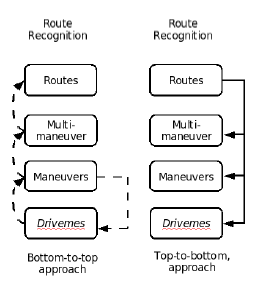
\includegraphics[width=.75\textwidth]{image/HMM_flowchart}
\caption{Hierarchy among the units of route recognition (Sathyanarayana et al., 2008)}
\end{figure}

In the Bottom-to-top approach, the maneuvers are the smallest unit to be recognized by the algorithms. The driver behavior can be discovered from the recognized maneuvers and be used to build the maneuver models. The multi-maneuver models use the maneuvers model to be built and finally become a complete route. The Bottom-to-Top approach is to detect the distratcion of driver based on the comparison of the neutral state vehicle operation data in the known maneuvers.

\begin{figure}[hbt!]\centering
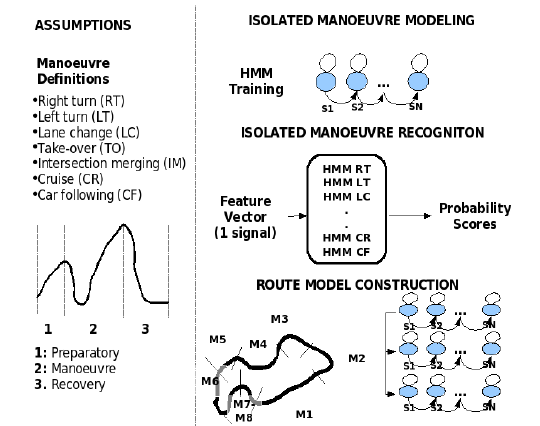
\includegraphics[width=.75\textwidth]{image/BottomtoTop}
\caption{Bottom-to-top approach for route model construction (Sathyanarayana et al., 2008)}
\end{figure}

In Top-to-Bottom approach, it is an opposite approach in driving behavior modeling. A single HMM is used to parse the route to the indvidual meaningful parts like maneuvers and states. The result of this approach is that the driver behavior in intersection will be identified by using three main clusters. The Top-to-Bottom approach is to recognized the route based on the vehicle operation data.

\begin{figure}[hbt!]\centering
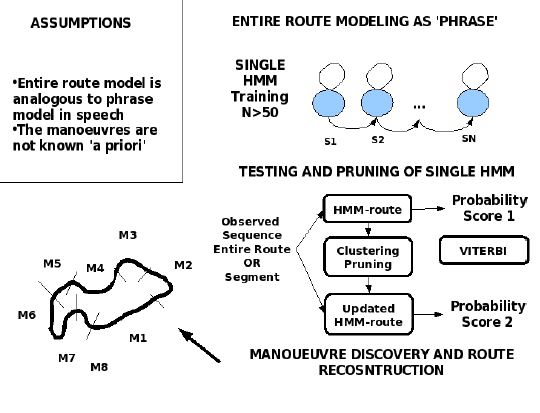
\includegraphics[width=.75\textwidth]{image/ToptoBottom}
\caption{Top-to-bottom approach for route model construction (Sathyanarayana et al., 2008)}
\end{figure}

\subsection{Data Collection}
The proposed method used UTDrive Vehicle to collect the data. The UTDrive Vehicle is converted from a Toyota RAV4 vehicle. The UTDrive Vehicle is equiped camera to capture the driver and the road. The driver speech also been recorded by the equiped microphone in the vehicle. Distance sensor using laser and GPS for position measurement are also equiped. The CAN-Bus is used to collected the vehicle speed, steering wheel angle, and brake/gas information. The vehicle also equiped gas/brake pedal pressure sensors. 

The experiment conducted in two different areas in order to collect two different senarios data. The residential and commercial area including the right turn, left turn and lane change were selected for drivers to driver through. The drivers were required to drive two times with neutral driving and distracted driving. 
 
\subsection{Conclusion}
Three different types of maneuvers (left turn, right turn, and lane change) were recognized by using the three CAN-Bus signals (vehicle speed, steering angle, and brake force). On the other hand, the distraction detection was well recognized and having 95\% accuracy.


\section{Driving Behavior Analysis Based on Vehicle OBD Information and AdaBoost Algorithms}
This paper was proposed by Shi-Huang et al.(2015). The researchers analyzed the drivers' behavior based on the on board diagnostic (OBD) information and using the AdaBoost Alogorithms to create the driving  behavior classification.Finally, the experimental results show the correctness of the proposed driving behavior analysis method has 99.8\% accuracy rate in various driving simulations.

\begin{figure}[hbt!]\centering
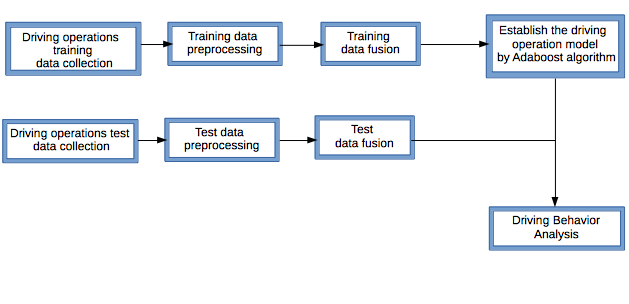
\includegraphics[width=.75\textwidth]{image/adaboost_flowchart}
\caption{The flowchart of the proposed driving behavior analysis method.}
\end{figure}

\subsection{AdaBoost Algorithms}
AdaBoost is a classification machine learning algorithm. The AdaBoost algorithms is to form a strong classifier by combining the a large number of weak classifier. There are three different types of AdaBoost algorithms. They are Gentle AdaBoost, Modest AdaBoost and Real AdaBoost.

\subsection{Driving Behaviour Analysis Method}
This proposed method used the OBD-II ssytem in the vehicle and EZ-SCAN5 as the OBD-II to Bluetooth adapter to collect the vehicle operation information. OBD-II is proposed in 1996 to replace the OBD-I system. The OBD-II system is implemented in every vehicle uncer the Environmental Protection Agency (EPA) regulation in USA since 1996. When the air-pollution contents exhausted by the vehicle exceed teh minimum level,the OBD-II system of the particular vehicle will generate the Diagnostic Trouble Code (DTC) message and Check Engine light will display on the vehicle dashboard. In order to communicate with the OBD-II system of the vehicle, EZ-SCAN5 as a OBD-II to Bluetooth adapter is required. The EZ-SCAN5 support most of the OBD-II communication protocols, such as SAE J1850 PWM, SAE J1850 VPW, ISO 9141-2, ISO 14230-4 KWP, and ISO 15765-4 CAN. If the communication protocol of the OBD-II system is not supported by the adapter, the vehicle operation information will not be able to retrieve.

This proposed method collected vehicle speed, engine speed(RPM), throttle position and engine load as the vehicle operation information. According to the engine characteristic curve, the proposed method developed two criteria for the data collection.

\begin{enumerate}
\item The normal vehicle condition data \\
The relative ratio of the vehicle speed and the engine speed is remained in a range that between 0.9 and 1.3. The result was tested in the same gear. The relative ratio of the engine speed and throttle valve is remained in a range that between 0.9 and 1.3. The engine load is remained between 20\% and 50\%.  
\item The bad vehicle condition data \\
The relative ratio of the vehicle speed and the engine speed is out of the range that between 0.9 and 1.3. The result was tested in the same gear. The relative ratio of the engine speed and throttle valve is out of the range that between 0.9 and 1.3. The engine load is out of the range that between 20\% and 50\%.
\end{enumerate}

\subsection{Vehicle OBD information Data Preprocessing}
The proposed method used three characteristics. The three characteristics are the relative ratio of the vehicle speed and engine speed, the relative ratio of throttle position and engine speed, and engine load. Using the characteristics to analyzed the current state of the driving behavior whether the driver is in safe state or dangerous state.The proposed method needed to compute the change rate of vehicle speed, engine speed and throttle position in the first step. The calculation shown in Equation\eqref{eqa:ada_change_rate}, where $t_{2} - t_{1} = 1$.\\
\begin{equation}
\label{eqa:ada_change_rate}
D(t) = \dfrac{data(t_{2})-data(t_{1})}{t_{2}-t_{1}}
\end{equation}

The next step is to calculate the relative ratio of the vehicle speed and engine speed, and the relative ratio of the throttle position and engine speed. The calculation shown in the Equation\eqref{eqa:ada_relative_eng_veh} and \eqref{eqa:ada_relative_eng_thr}. \\
\begin{equation}
\label{eqa:ada_relative_eng_veh}
R_{cz}(t) = \dfrac{cs(t)}{220} \div \dfrac{zs(t)}{8000}
\end{equation}
\\
where $R_{cz}(t)$ is the relative ratio of engine speed and vehicle speed. $cs(t)$ is the vehicle speed at time $t$. The 220 is the value of maximum vehicle speed. $zs(t)$ is the engine speed a time $t$. The 8000 is the value of maximum engine speed of the vehicle.\\

\begin{equation}
\label{eqa:ada_relative_eng_thr}
R_{jz}(t) = \dfrac{jq'(t)}{max(jq')} \div \dfrac{zs'(t)}{max(zs'(t))}
\end{equation}
\\
where $R_{jz}(t)$ is the relative ratio of engine speed and throttle position. The $jq'(t)$ is the change rate of the throttle position at time $t$. $zs'(t)$ is the change rate of the engine speed at time $t$. The $max(jq'(t))$ and $max(zs'(t))$ is the maximum value of the change rate of throttle position and engine speed, respectively.\\

Based on the two computed features and engine load, this three features were combined to determine the vehicle data is normal or bad driving behavior.

\subsection{Experimental Results}
The proposed method used the tookit-GML-AdaBoost-matlab of MATLAB to execute data preprocessing and driving behavior modeling. The preprocessed data is tested on three diferent types of the AdaBoost algorithms. They are Gentle AdaBoost, Modest AdaBoost and Real AdaBoost. The Real AdaBoost are better than other AdaBoost algorithms with the highest accuracy rate, 99.8\%.